%%%%%%%%%%%%%%%%%%%%%%%%%%%%%%%%%%%%%%%%%
% Jacobs Landscape Poster
% LaTeX Template
% Version 1.0 (29/03/13)
%
% Created by:
% Computational Physics and Biophysics Group, Jacobs University
% https://teamwork.jacobs-university.de:8443/confluence/display/CoPandBiG/LaTeX+Poster
% 
% Further modified by:
% Nathaniel Johnston (nathaniel@njohnston.ca)
%
% This template has been downloaded from:
% http://www.LaTeXTemplates.com
%
% License:
% CC BY-NC-SA 3.0 (http://creativecommons.org/licenses/by-nc-sa/3.0/)
%
%%%%%%%%%%%%%%%%%%%%%%%%%%%%%%%%%%%%%%%%%

%----------------------------------------------------------------------------------------
%	PACKAGES AND OTHER DOCUMENT CONFIGURATIONS
%----------------------------------------------------------------------------------------

\documentclass[final]{beamer}

\usepackage[scale=1.24]{beamerposter} % Use the beamerposter package for laying out the poster

\usetheme{confposter} % Use the confposter theme supplied with this template

\setbeamercolor{block title}{fg=ngreen,bg=white} % Colors of the block titles
\setbeamercolor{block body}{fg=black,bg=white} % Colors of the body of blocks
\setbeamercolor{block alerted title}{fg=white,bg=dblue!70} % Colors of the highlighted block titles
\setbeamercolor{block alerted body}{fg=black,bg=dblue!10} % Colors of the body of highlighted blocks
% Many more colors are available for use in beamerthemeconfposter.sty

%-----------------------------------------------------------
% Define the column widths and overall poster size
% To set effective sepwid, onecolwid and twocolwid values, first choose how many columns you want and how much separation you want between columns
% In this template, the separation width chosen is 0.024 of the paper width and a 4-column layout
% onecolwid should therefore be (1-(# of columns+1)*sepwid)/# of columns e.g. (1-(4+1)*0.024)/4 = 0.22
% Set twocolwid to be (2*onecolwid)+sepwid = 0.464
% Set threecolwid to be (3*onecolwid)+2*sepwid = 0.708

\newlength{\sepwid}
\newlength{\onecolwid}
\newlength{\onepointfivecolwid}
\newlength{\twocolwid}
\newlength{\threecolwid}
\setlength{\paperwidth}{46.81in} % A0 width: 46.8in
\setlength{\paperheight}{33.11in} % A0 height: 33.1in
\setlength{\sepwid}{0.02\paperwidth} % Separation width (white space) between columns
\setlength{\onecolwid}{0.22\paperwidth} % Width of one column
\setlength{\onepointfivecolwid}{0.33\paperwidth}
\setlength{\twocolwid}{0.464\paperwidth} % Width of two columns
\setlength{\threecolwid}{0.708\paperwidth} % Width of three columns
\setlength{\topmargin}{-0.5in} % Reduce the top margin size
%-----------------------------------------------------------

\usepackage{graphicx}  % Required for including images

\usepackage{booktabs} % Top and bottom rules for tables

\usepackage[most]{tcolorbox}

%----------------------------------------------------------------------------------------
%	TITLE SECTION 
%----------------------------------------------------------------------------------------

\title{Emergent Communication in a Multi-modal, Multi-step Referential Game} % Poster title

\author{Katrina Evtimova\inst{1} \and Andrew Drozdov\inst{2} \and Douwe Kiela\inst{3} \and Kyunghyun Cho\inst{1,2,3,4}} % Author(s)

\institute[affiliations]{\inst{1} Center for Data Science, New York University \inst{2} Department of Computer Science, New York University \\ \inst{3} Facebook AI Research \inst{4} CIFAR Azrieli Global Scholar} % Institution(s)

%----------------------------------------------------------------------------------------

\begin{document}

\addtobeamertemplate{block end}{}{\vspace*{0.5ex}} % White space under blocks
\addtobeamertemplate{block alerted end}{}{\vspace*{0.5ex}} % White space under highlighted (alert) blocks

\setlength{\belowcaptionskip}{0.5ex} % White space under figures
\setlength\belowdisplayshortskip{0.5ex} % White space under equations

\addtobeamertemplate{headline}{} 
{
\begin{tikzpicture}[remember picture,overlay] 
\node [shift={(-22 cm,-10cm)}] at (current page.north east) {
\includegraphics[height=3cm]{logos/AI-logo}}; 
\end{tikzpicture} 
}
\addtobeamertemplate{headline}{} 
{
\begin{tikzpicture}[remember picture,overlay] 
\node [shift={(-10 cm,-10cm)}] at (current page.north east) {
\includegraphics[height=3cm]{logos/fair-wordmark-style-1}}; 
\end{tikzpicture} 
}
\addtobeamertemplate{headline}{} 
{
\begin{tikzpicture}[remember picture,overlay] 
\node [shift={(10 cm,-10cm)}] at (current page.north west) {

\includegraphics[height=3cm]{logos/nyu_short_color}
}; 
\end{tikzpicture} 
}

\addtobeamertemplate{headline}{} 
{
\begin{tikzpicture}[remember picture,overlay] 
\node [shift={(-14 cm,6cm)}] at (current page.south east) {
\begin{tcolorbox}[colback=blue!5!white,colframe=blue!75!black,width=\onecolwid]
  \begin{minipage}{.3\textwidth}
  
\includegraphics[width=\textwidth]{links/qr_code_blue_bg}
  \end{minipage} \quad
  \begin{minipage}{.6\textwidth}
  {\normalsize
  Code (Github) \\
\href{https://github.com/nyu-dl/MultimodalGame}{nyu-dl/MultimodalGame}
  }
  \end{minipage}
  \end{tcolorbox}
}; 
\end{tikzpicture} 
}

\addtobeamertemplate{headline}{} 
{
\begin{tikzpicture}[remember picture,overlay] 
\node [shift={(16.5 cm,6cm)}] at (current page.south west) {
  \begin{tcolorbox}[colback=blue!5!white,colframe=blue!75!black,width=\onecolwid]
  \begin{minipage}{.3\textwidth}
  
\includegraphics[width=\textwidth]{links/qr_code_blue_bg}
  \end{minipage} \quad
  \begin{minipage}{.6\textwidth}
  {\normalsize
    Paper (arXiv) \\
    \href{https://arxiv.org/abs/1705.10369}{1705.10369}
  }
  \end{minipage}
  \end{tcolorbox}
}; 
\end{tikzpicture} 
}

\begin{frame}[t] % The whole poster is enclosed in one beamer frame

\begin{columns}[t] % The whole poster consists of three major columns, the second of which is split into two columns twice - the [t] option aligns each column's content to the top

\begin{column}{\sepwid}\end{column} % Empty spacer column

\begin{column}{\onecolwid} % The first column

%----------------------------------------------------------------------------------------
%	OBJECTIVES
%----------------------------------------------------------------------------------------

\begin{block}{Overview}

This works presents a novel referential game where the sender and receiver are grounded in two separate modalities, have an adaptive conversation length, and learn a communication protocol.

\vspace{5mm}

We find that the agents vary conversation length according to the difficulty of the task and gradual information exchange informs better predictions.

\end{block}

\vspace{5mm}

\begin{block}{Referential Games}

\vspace{-15mm}

\begin{center}
% 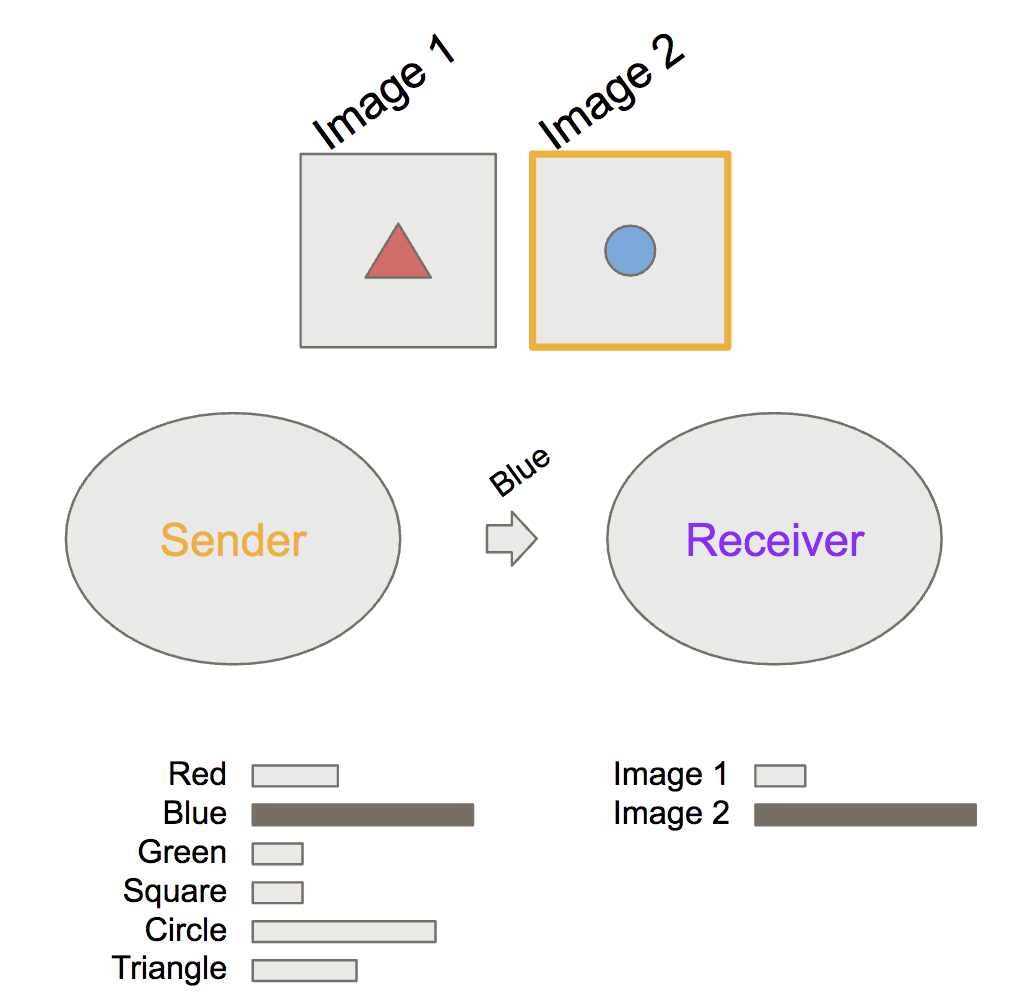
\includegraphics[width=0.8\linewidth]{figures/lazaridou}
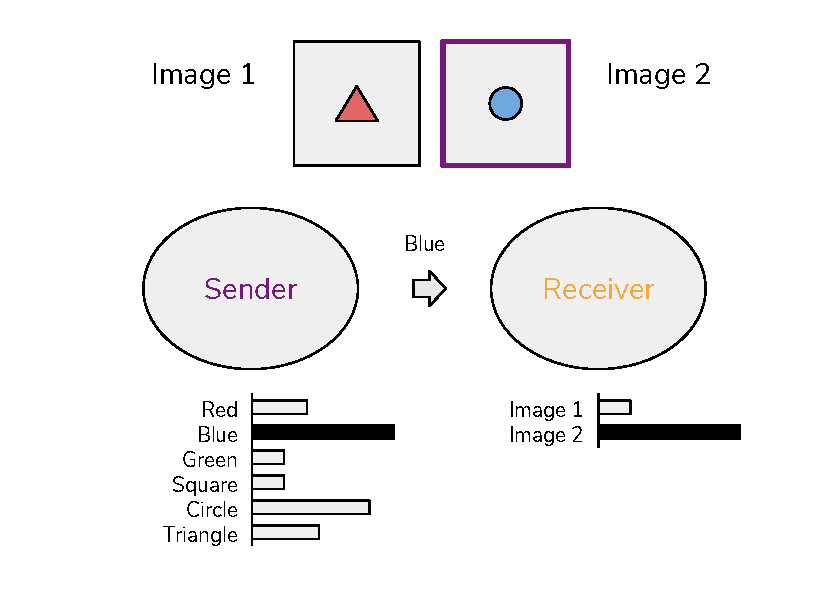
\includegraphics[width=0.8\linewidth]{/Users/adrozdov/Downloads/ref_game_lazaridou.pdf}
\end{center}

\vspace{5mm}

An example Referential Game where both agents see the images, the Sender knows the target image, and it may send one message to the Receiver \cite{Lazaridou:2017multi}.

\vspace{5mm}

Other setups have been studied such as one where the Sender and Receiver have a conversation of fixed length, the Receiver may send a single discrete token from a small vocabulary, and the Sender may only answer yes or no \cite{Jorge:2016learning}.

\end{block}

\vspace{5mm}

% \begin{tcolorbox}[colback=blue!5!white,colframe=blue!75!black]
% % \vspace{5mm}

% \begin{minipage}{.3\textwidth}
% 
\includegraphics[width=\textwidth]{links/qr_paper_blue_bg}
% \end{minipage} \quad
% \begin{minipage}{.6\textwidth}
%   Paper (arXiv) \\
%   \href{https://arxiv.org/abs/1705.10369}{1705.10369}
% \end{minipage}

% %   \centering
% %   Code \\
% %   \href{https://github.com/nyu-dl/MultimodalGame}{https://github.com/nyu-dl/MultimodalGame}

% %   \vspace{5mm}
  
% %   \centering
% %   Paper \\
% %   \href{https://arxiv.org/abs/1705.10369}{https://arxiv.org/abs/1705.10369}
  
% % \vspace{5mm}
% \end{tcolorbox}

%------------------------------------------------

% \begin{figure}
% \includegraphics[width=0.8\linewidth]{figures/step0002.jpg}
% \caption{Architecture of Ping}
% \end{figure}

%----------------------------------------------------------------------------------------

\end{column} % End of the first column

\begin{column}{\sepwid}\end{column} % Empty spacer column

\begin{column}{\onecolwid}


\begin{block}{This Work}

\begin{center}
% 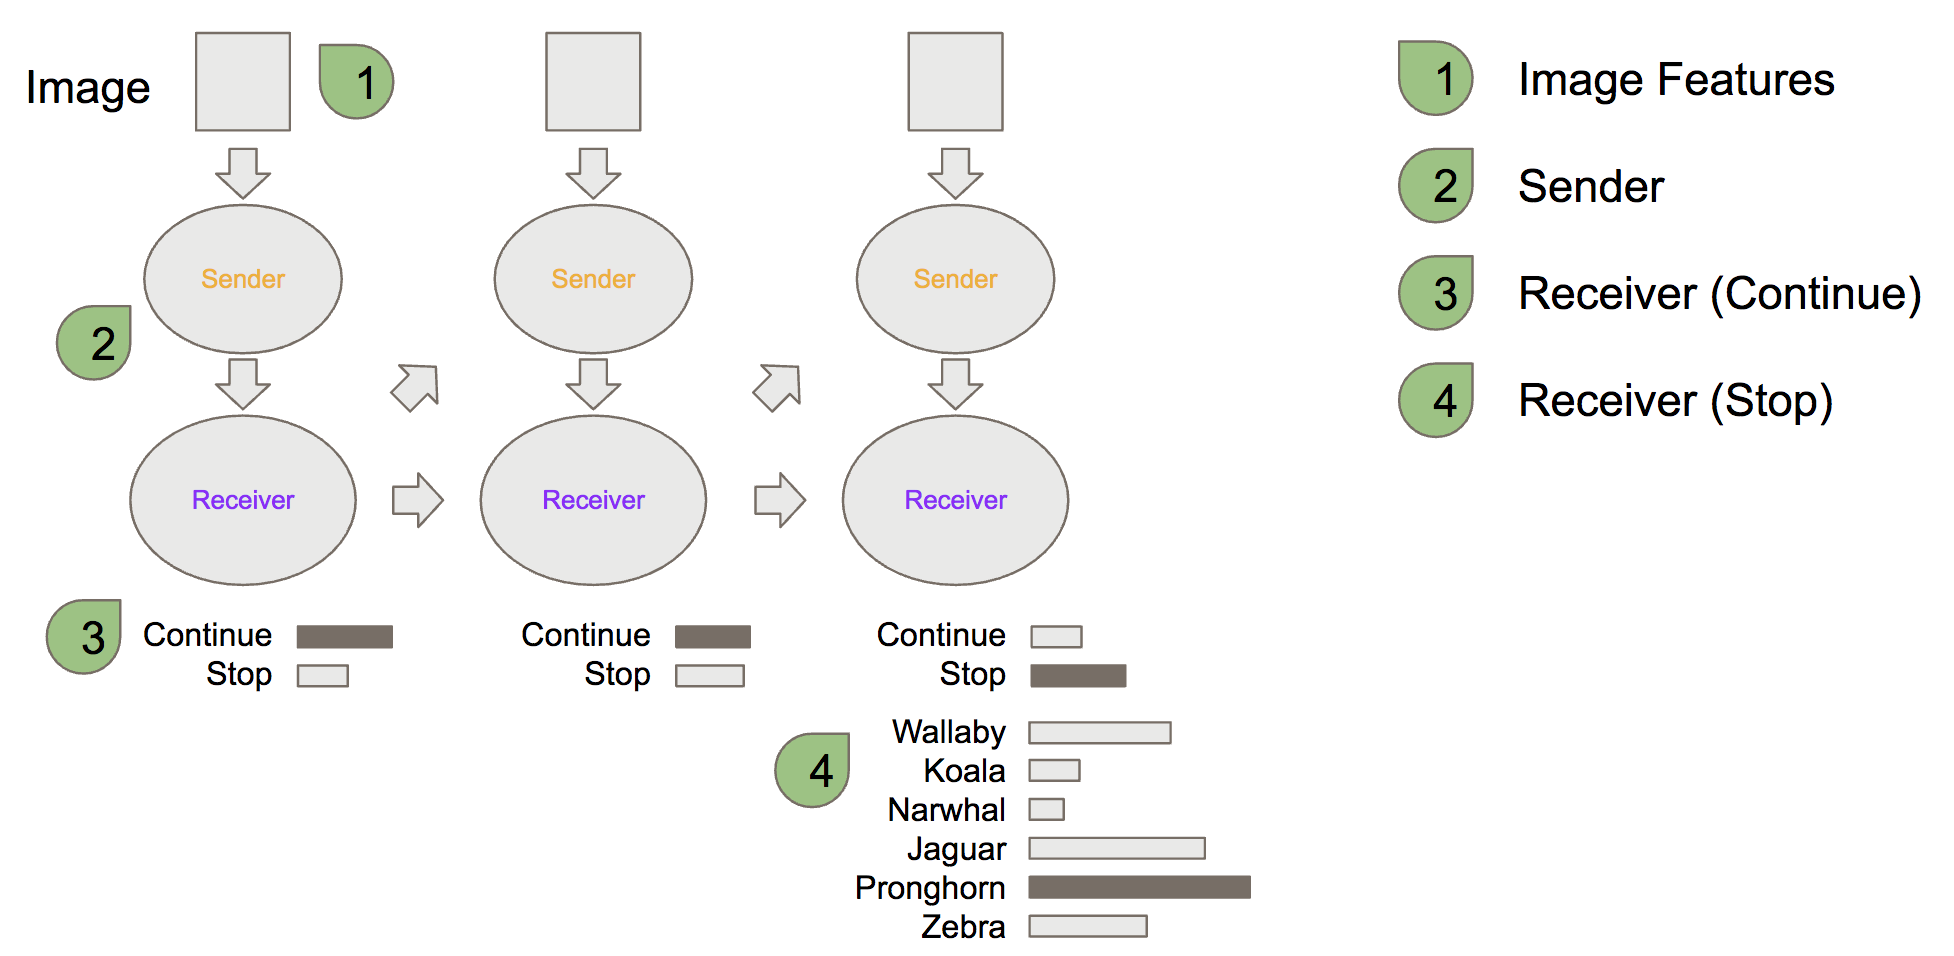
\includegraphics[width=0.8\linewidth]{figures/mmg}
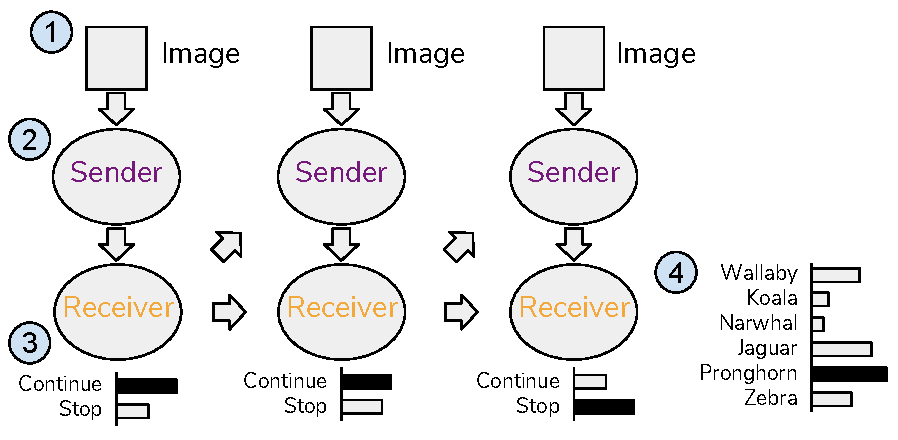
\includegraphics[width=0.8\linewidth]{/Users/adrozdov/Downloads/ref_game_evtimova_2.pdf}
\end{center}

\begin{enumerate}
\item[1.] The image features are extracted using a pre-trained network.
\item[2.] The Sender incorporates the image and the Receiver's message (if it's available) to generate a message for the Receiver.
\item[3.] The Receiver incorporates the class descriptors, the Sender's message, and its own hidden state to generate a message for the Sender.
\item[4.] When the conversation terminates, the Receiver predicts the image's most likely class.
\end{enumerate}

\vspace{22mm}

\textbf{Per-Instance Loss:}

\begin{align*}
L^i &= L^i_{c} + L^i_{r} - H^i_{stop,sen,rec}
\end{align*}

\begin{itemize}
\item $L^i_{c}$ is the classification loss.
\item $L^i_{r}$ is the reinforcement learning loss.
\item $H^i_{stop,sen,rec}$ is the entropy regularization on the Sender's messages, the Receiver's messages, and the Receiver's stop-bit.
\end{itemize}

\end{block}

\begin{block}{Experimental Setup}

\textbf{In-Domain:} 60 mammals with 550 images per mammal for training, 50 validation, and 20 test.

\textbf{Out-of-Domain:} 10 mammals with 20 images.

\textbf{Transfer:} 10 insects with 100 images.

\end{block}

\end{column} % End of the second column

% % % % 

\begin{column}{\sepwid}\end{column} % Empty spacer column

\begin{column}{\twocolwid} % The third column

\begin{block}{Results}

\begin{minipage}{\textwidth}
\centering
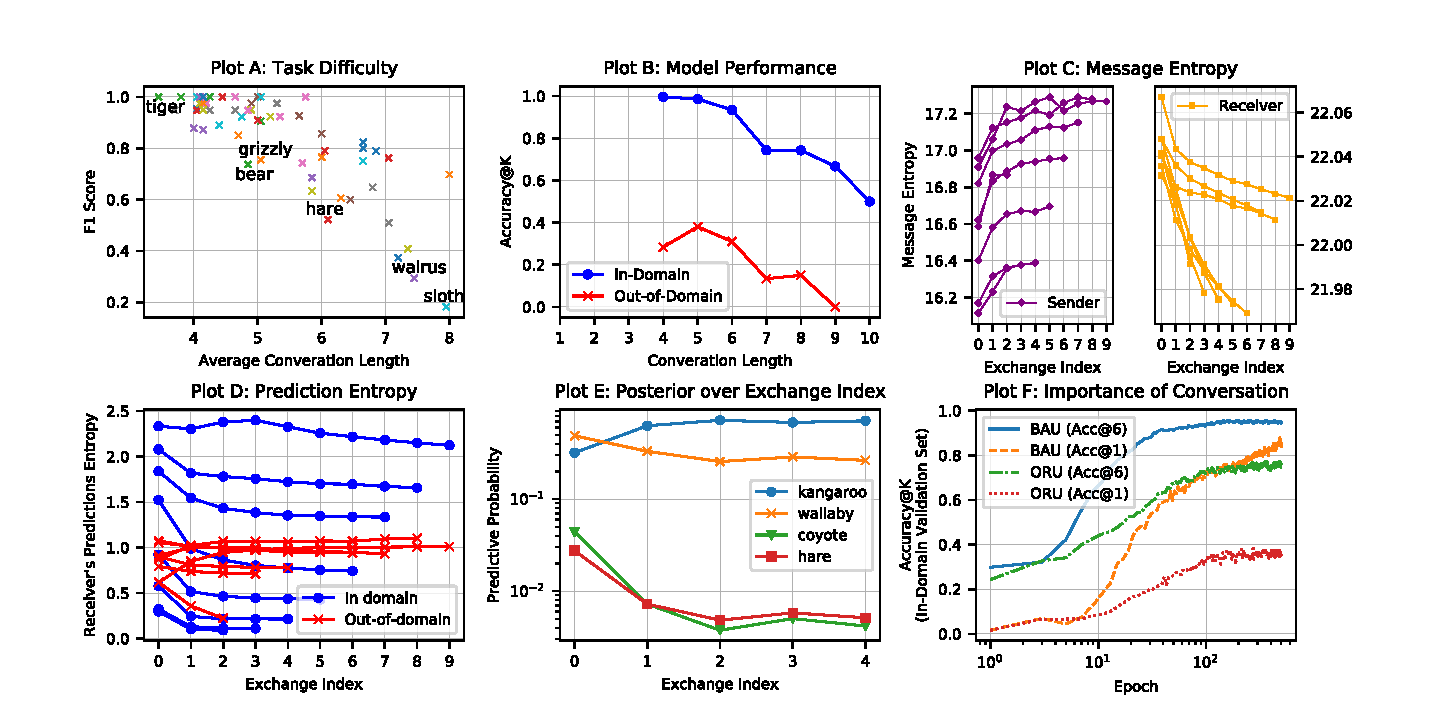
\includegraphics[width=\textwidth]{/Users/adrozdov/Research/MultimodalGame-Private/poster_figures.pdf}
\end{minipage}

% \begin{minipage}{.3\textwidth}
%   \centering
%   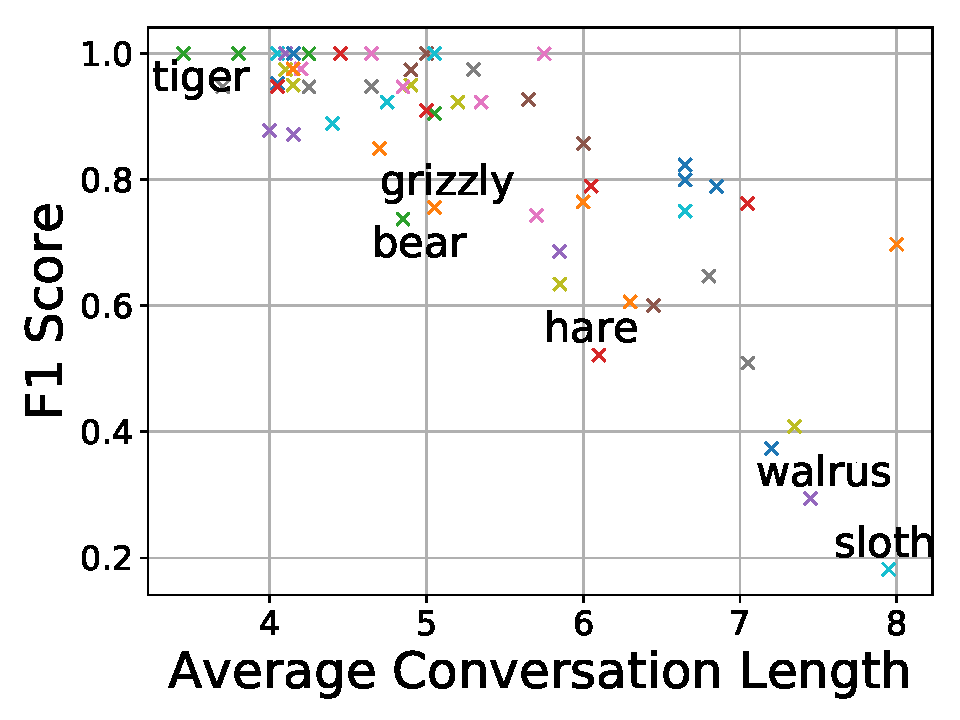
\includegraphics[width=\textwidth]{figures/corr_conv_len_difficulty}
% \end{minipage} \quad
% \begin{minipage}{.3\textwidth}
%   \centering
%   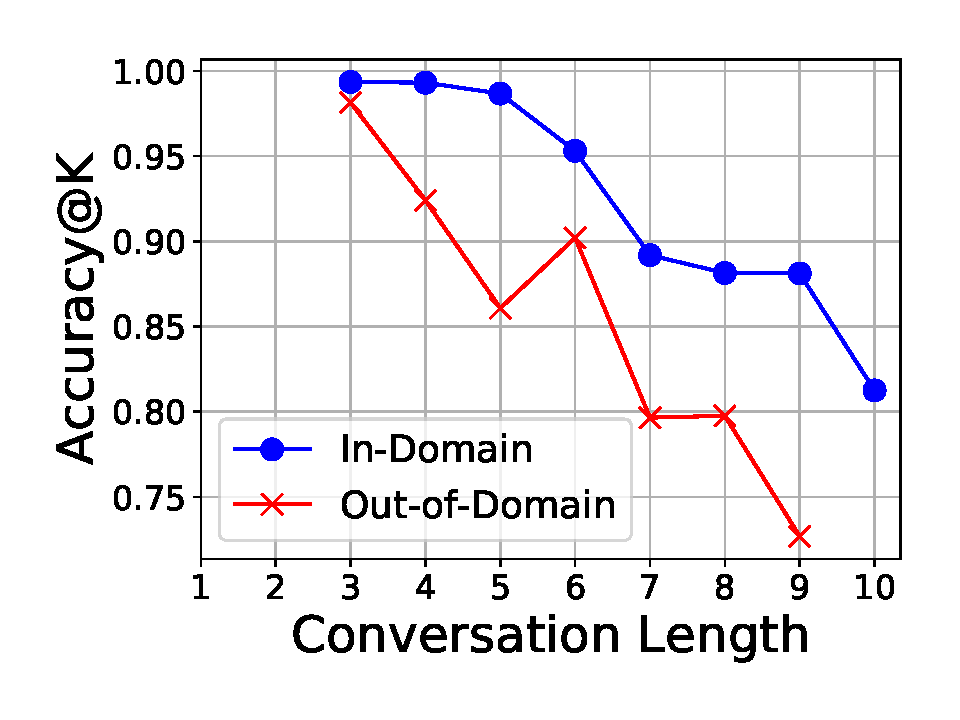
\includegraphics[width=\textwidth]{figures/acc_top-6_adaptive_conv-len_in_out-line}
% \end{minipage}
% \begin{minipage}{.3\textwidth}
%   \centering
%   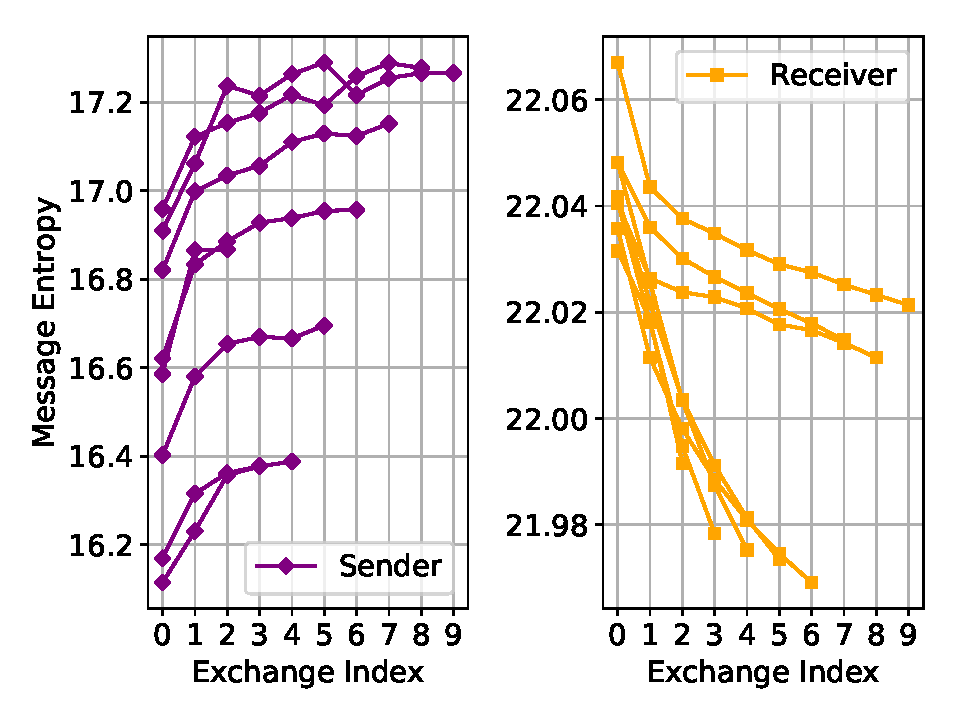
\includegraphics[width=\textwidth]{figures/SR_msg_entropy_adaptive_indomain_pt_best_02}
% \end{minipage}

% \vspace{5mm}

% \begin{minipage}{.3\textwidth}
%   \centering
%   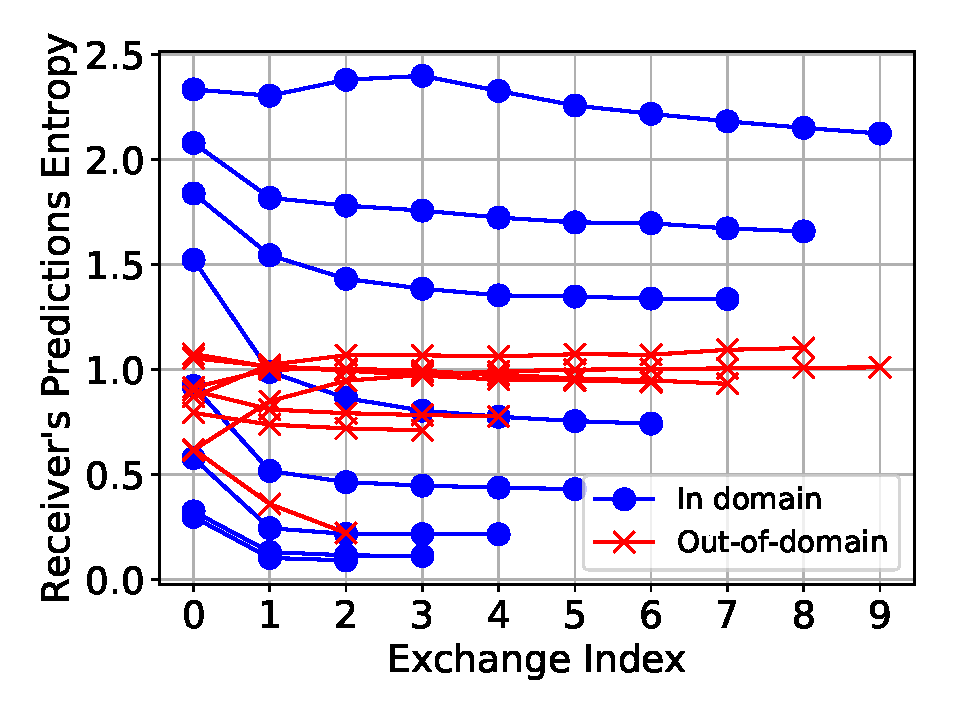
\includegraphics[width=\textwidth]{figures/R_pred_entropy_adaptive_in_out_big.pdf}
% \end{minipage} \quad
% \begin{minipage}{.3\textwidth}
%   \centering
%   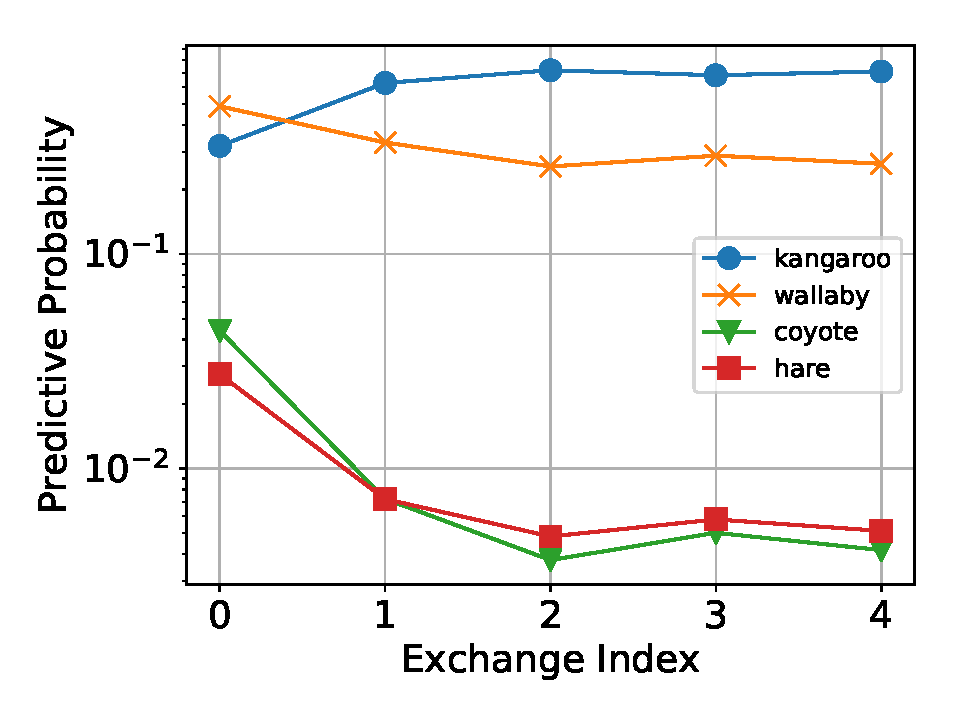
\includegraphics[width=\textwidth]{figures/mammal_kangaroo}
% \end{minipage} \quad
% \begin{minipage}{.3\textwidth}
%   \centering
%   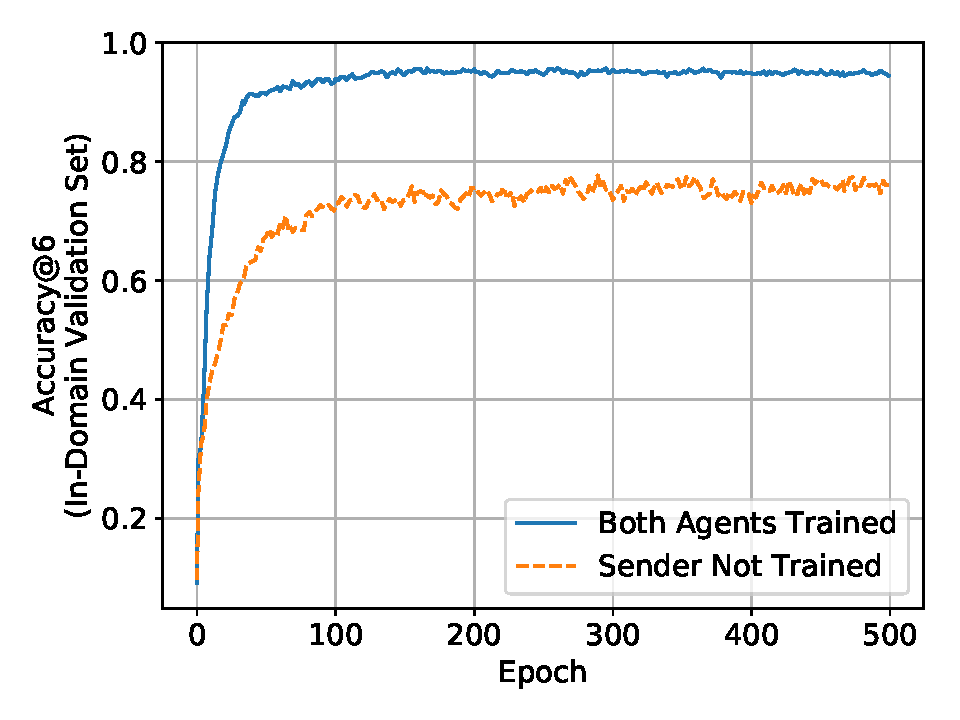
\includegraphics[width=\textwidth]{figures/sender_not_trained}
% \end{minipage}

% \vspace{5mm}

% \begin{minipage}{.475\textwidth}
% The performance correlates with the difficulty of the task.
% \end{minipage} \quad
% \begin{minipage}{.475\textwidth}
% % The performance correlates with the difficulty of the task.
% \end{minipage}

\end{block}

\begin{columns}[t,totalwidth=\twocolwid] % Split up the two columns wide column again

\begin{column}{\onecolwid} % The first column within column 2 (column 2.1)



\begin{block}{Analysis}

\begin{itemize}
\item There's a significant negative relationship between class difficulty and the average conversation length [Plot A].
\item Examples for which conversations are shorter are better classified [Plot B].
\item As the conversation progress, the Receiver's messages become more specific [Plot C right] and the Sender's messages become less certain [Plot C left].
\item The conversation length correlates well with the Receiver's prediction confidence [Plot D].
\item As the Receiver gathers more information, similar but incorrect categories receive smaller probabilities than the correct one [Plot E].
\item The learned protocol was more effective when communication was bidirectional [Plot F].
\end{itemize}

\end{block}

%----------------------------------------------------------------------------------------

\end{column} % End of column 2.1

\begin{column}{\onecolwid} % The second column within column 2 (column 2.2)

\begin{block}{References}

% {\small
% [Lazaridou et al., 2016] Lazaridou, Angeliki and Peysakhovich, Alexander and Baroni, Marco (2016). \\
% Multi-agent cooperation and the emergence of (natural) language. \\
% \href{https://arxiv.org/abs/1612.07182}{In Proceedings of ICLR}

% \vspace{5mm}

% [Jorge et al., 2016] Jorge, Emilio and K{\aa}geb{\"a}ck, Mikael and Gustavsson, Emil (2016). \\
% Learning to Play Guess Who? and Inventing a Grounded Language as a Consequence. \\
% \href{https://arxiv.org/abs/1611.03218}{arXiv preprint arXiv:1611.03218}
% }

\nocite{*} % Insert publications even if they are not cited in the poster
\footnotesize{\bibliographystyle{apalike}
\bibliography{main}\vspace{0.75in}}

\end{block}

\end{column} % End of column 2.2

\end{columns} % End of the split of column 2



\end{column} % End of the third column

\end{columns} % End of all the columns in the poster

\end{frame} % End of the enclosing frame

\end{document}
